\documentclass[a4paper,12pt]{article}
% The same source supports pdfLaTeX, XeLaTeX, LuaLaTeX and Tectonic.
\usepackage{iftex}
\ifPDFTeX
  \usepackage[T1,T2A]{fontenc}
  \usepackage[utf8]{inputenc}
  \usepackage{tgtermes}
  \DeclareFontFamilySubstitution{T2A}{\rmdefault}{Tempora-TLF}
\else
  \usepackage{fontspec}
  \IfFontExistsTF{Times New Roman}
    {\setmainfont{Times New Roman}}
    {\setmainfont{cmunrm.otf}[BoldFont=cmunbx.otf,
      ItalicFont=cmunti.otf,BoldItalicFont=cmunbi.otf]
      \AtBeginDocument{\setlength{\emergencystretch}{4em}}}
  \IfFontExistsTF{Arial}
    {\setsansfont{Arial}}
    {\setsansfont{cmunss.otf}[BoldFont=cmunsx.otf,
      ItalicFont=cmunsi.otf,BoldItalicFont=cmunso.otf]}
  \IfFontExistsTF{Menlo}
    {\setmonofont{Menlo}[Scale=0.82]}
    {\setmonofont{cmuntt.otf}[BoldFont=cmuntb.otf,
      ItalicFont=cmunit.otf,BoldItalicFont=cmuntx.otf,Scale=0.82]}
\fi
\usepackage[russian]{babel}
\usepackage{amsmath,amssymb,amsthm,mathtools}
\usepackage[left=25mm,right=20mm,top=20mm,bottom=22mm]{geometry}
\usepackage{setspace,indentfirst,enumitem,booktabs,array,graphicx,needspace,float}
\usepackage{caption}
\graphicspath{{figures/}{paper/figures/}{output/pdf/figures/}}
\usepackage{microtype}
\usepackage[unicode,hidelinks]{hyperref}
\hypersetup{pdftitle={Гиперболическое сингулярное разложение (HSVD) и приложения},pdfauthor={},pdfsubject={Теоретические свойства, алгоритм и приложения},pdfkeywords={гиперболическое сингулярное разложение, неопределённая (индефинитная) метрика, численный ранг, обусловленность, устойчивость, гиперболический метод Якоби}}
\setstretch{1.18}
\setlength{\parindent}{1.25cm}
\setlength{\parskip}{0pt}
\clubpenalty=10000
\widowpenalty=10000
\displaywidowpenalty=10000
\setlength{\emergencystretch}{2em}
\setlist{itemsep=2pt,topsep=4pt,parsep=0pt}
\captionsetup{font=small,labelfont=bf,labelsep=period}
\renewcommand{\arraystretch}{1.15}
\DeclareMathOperator{\rank}{rank}
\DeclareMathOperator{\diag}{diag}
\DeclareMathOperator{\sign}{sign}
\newtheoremstyle{csstyle}{6pt}{6pt}{\normalfont}{}{\bfseries}{.}{\newline}{}
\theoremstyle{csstyle}
\newtheorem{theorem}{Теорема}[section]
\newtheorem{lemma}[theorem]{Лемма}
\newtheorem{proposition}[theorem]{Утверждение}
\newtheorem{corollary}[theorem]{Следствие}
\newtheorem{definition}[theorem]{Определение}
\newtheorem{example}[theorem]{Пример}
\newcommand{\code}[1]{\texttt{\detokenize{#1}}}
\DeclareMathOperator{\im}{Im}
\DeclareMathOperator{\nnz}{nnz}
\newcommand{\R}{\mathbb R}
\newcommand{\HSVDComplex}{\mathbb C}
\newtheorem*{witt}{Теорема Витта}
\usepackage{etoolbox}
\AtBeginEnvironment{lemma}{\Needspace{5\baselineskip}}
\AtBeginEnvironment{proposition}{\Needspace{6\baselineskip}}
\AtBeginEnvironment{theorem}{\Needspace{8\baselineskip}}
\AtBeginEnvironment{example}{\Needspace{6\baselineskip}}
\AtBeginEnvironment{proof}{\Needspace{3\baselineskip}}
\pretocmd{\section}{\Needspace{7\baselineskip}}{}{}
\raggedbottom
\begin{document}
\hypersetup{pageanchor=false}
\begin{titlepage}
\centering
\vspace*{4.4cm}
{\LARGE\bfseries Гиперболическое сингулярное разложение (HSVD) и приложения\par}
\vspace{2cm}
\begin{minipage}{0.86\textwidth}
\centering
\textbf{Ключевые слова:} гиперболическое сингулярное разложение, неопределённая (индефинитная) метрика, численный ранг, обусловленность, устойчивость, гиперболический метод Якоби.
\end{minipage}
\end{titlepage}
\hypersetup{pageanchor=true}
\setcounter{page}{2}

\section*{Аннотация}
Рассматривается HSVD произвольной прямоугольной матрицы.
Приведены два доказательства известной теоремы существования: через теорему
Витта и конструктивное. Исследованы ранги степеней и жорданова структура
вспомогательной матрицы, ограничения сигнатуры, минимальность числа
ненулевых элементов канонической формы.
Изучена локальная постоянность параметра $j=\rank(A)-\rank(AJA^*)$.
Получены оценки точности гиперболических сингулярных чисел,
чувствительности собственных векторов и обратной ошибки по невязкам.
Выделены причины роста нормы матрицы $V$ и оценена сложность алгоритма.

Описаны общий вычислительный алгоритм, программная реализация и
воспроизводимые эксперименты. Рассмотрены приложения к сравнению
данных с фоном, методу наименьших квадратов с неопределённой метрикой и сжатию матрицы Грама.
Для задачи наименьших квадратов дан критерий существования минимума,
а для сжатия матрицы Грама получена оценка погрешности.
На открытых данных об измерениях белков построены проекции PCA и cPCA.
Результат вычисления через HSVD проверен прямой диагонализацией
матрицы разности ковариаций.

\vspace{0.5cm}
\noindent\textbf{Классификация ACM CCS 2012}\par
\begin{itemize}[leftmargin=1.4em,itemsep=5pt]
\item Mathematics of computing $\sim$ Mathematical analysis $\sim$ Numerical analysis $\sim$ Computations on matrices.
\item Mathematics of computing $\sim$ Mathematical software.
\item Software and its engineering $\sim$ Software creation and management $\sim$ Software verification and validation $\sim$ Software defect analysis $\sim$ Software testing and debugging.
\end{itemize}
Классификация оформлена по правилам ACM~\cite{ACM}.


\newpage
\tableofcontents
\newpage

\section*{Введение}
\phantomsection
\addcontentsline{toc}{section}{Введение}

Сингулярное разложение матрицы (SVD) имеет большое теоретическое и практическое значение. Оно широко используется при решении задач методом наименьших квадратов, построении низкоранговых приближений, сжатии данных и обработке изображений \cite{Kalman}.
Известно множество алгоритмов, позволяющих эффективно вычислять SVD произвольной матрицы \cite{Golub}.

Однако классическое SVD естественным образом связано с евклидовыми пространствами, то есть с линейными пространствами, в которых скалярное произведение является положительно определённым. В некоторых задачах возникает необходимость рассматривать более общий случай пространств с неопределённым (индефинитным) скалярным произведением \cite{BOS, ILS, ShirokovYM}. В такой ситуации естественно рассматривать соответствующее обобщение SVD -- гиперболическое сингулярное разложение (HSVD), одна из общих формулировок которого приведена в работе \cite{BOS}.

\textbf{Актуальность темы.} В отличие от классического SVD, для которого существует очень развитая теория и множество вычислительных методов, HSVD изучено значительно слабее. Это относится как к теоретическим вопросам, связанным со структурой разложения, так и к алгоритмам его вычисления. Поэтому исследование различных подходов к построению HSVD, их реализация и численное сравнение представляют самостоятельный интерес.

\textbf{Цель исследования.} Исследовать структуру HSVD в формулировке~\cite{Shirokov}, построить и реализовать алгоритм его вычисления для произвольных прямоугольных матриц, оценить точность результатов и сравнить алгоритм с гиперболическим методом Якоби.

\textbf{Задачи исследования.}
\begin{enumerate}
    \item Исследовать возможную структуру матрицы $\Sigma$. Провести доказательство существования HSVD.
    \item Исследовать чувствительность параметра $j=\rank(A)-\rank(AJA^*)$ и выяснить, когда он сохраняется при малых возмущениях матрицы $A$.
    \item Построить алгоритм вычисления матриц $U$, $\Sigma$, $V$ в общем случае, включая нейтральные блоки при $j>0$.
    \item Оценить точность гиперболических сингулярных чисел, чувствительность векторов разложения, связь невязок с обратной ошибкой и стоимость вычислений.
    \item Реализовать алгоритм и проверить его на матрицах различной структуры. На матрицах полного столбцового ранга сравнить точность и время работы с гиперболическим методом Якоби.
    \item Рассмотреть и реализовать приложения HSVD.
\end{enumerate}

\textbf{Объект и предмет исследования.}
\begin{itemize}
    \item \textbf{Объект:} гиперболическое сингулярное разложение матриц.
    \item \textbf{Предмет:} структура HSVD, алгоритм его вычисления и чувствительность результатов к возмущениям.
\end{itemize}


\section{Обзор литературы}
\label{sec:literature}
Одна из общих формулировок HSVD была предложена \textit{A.~W.~Bojanczyk, R.~Onn, A.~O.~Steinhardt} \cite{BOS}. Однако в данной формулировке матрица $\Sigma$ из гиперболического сингулярного разложения $A = U\Sigma V^*$ содержала комплексные элементы, а также $V$ могла быть псевдогиперобменной (т.~е. $V^*JV = \hat{J}$, где $J$ и $\hat{J}$ диагональные, причём матрица $J$ содержит на диагонали только $\pm 1$, а $\hat{J}$ содержит на диагонали только $\pm 1$ или $0$). \textit{H.~Zha} указывает на неестественность такого разложения и предлагает другую формулировку \cite{Zha}, содержащую вещественную матрицу $\Sigma$ и гиперобменную (hyperexchange) матрицу $V$, а также приводит более простое доказательство, лучше раскрывающее структуру гиперболического разложения и являющееся следствием более общего разложения для пар матриц $(A, B)$, где $A$ -- эрмитова, $B$ -- произвольная. Позднее \textit{B.~C.~Levy} приводит немного другую формулировку \cite{Levy}, имеющую более прямую конструкцию и не использующую разложение для пар матриц.

В работе \cite{Shirokov} \textit{D.~S.~Shirokov} приводит новую формулировку для HSVD, не использующую понятия гиперобменных матриц (вместо них используются более простые псевдоунитарные матрицы), а также избавляющую от излишних параметров в разложении, которые присутствовали в формулировке \textit{H.~Zha}. В статье доказывается теорема о существовании разложения в новой формулировке и приводится наивный алгоритм вычисления этого разложения.
Новая формулировка является более естественной и удобной для некоторых приложений \cite{ShirokovYM} по сравнению с предыдущими формулировками из-за отсутствия гиперобменных матриц.

Отдельное направление работ посвящено разработке численных алгоритмов для вычисления HSVD. Одним из первых подробно описанных алгоритмов является метод на основе гиперболических (или $J$-ортогональных) вращений Якоби, подробно рассмотренный, например, в работе~\cite{Jacobi}. Этот метод обобщает ранее известный метод ортогональных вращений Якоби~\cite{Golub}, позволяющий итеративно вычислять SVD произвольной матрицы $A$, приводя её к матрице с ортогональными столбцами с помощью преобразований специального вида (ортогональных вращений).

\textit{I.~Slapni\v{c}ar}~\cite{Jacobi} показал, что при определённых условиях на масштабированную матрицу метод Якоби позволяет вычислять гиперболические сингулярные числа с малой относительной погрешностью. Анализ этой работы относится к вещественным матрицам полного столбцового ранга. Точность вычисления векторов также зависит от того, насколько соответствующие собственные значения отделены от остальных. Эти теоретические результаты подтверждаются численными экспериментами, демонстрирующими, что гиперболический метод Якоби может надёжно восстанавливать даже очень малые гиперболические сингулярные числа.

Позднее \textit{V.~Novakovi\'c, S.~Singer} показали~\cite{GPU-HSVD}, что гиперболический алгоритм Якоби может быть существенно ускорен за счёт параллельных вычислений на графических процессорах (GPU). Авторы предлагают модифицированный алгоритм и описывают стратегию его параллельной реализации. Авторы исследуют производительность и точность GPU-реализации на выбранных тестах.

Существует также блочный аналог алгоритма Якоби для гиперболического случая, который рассмотрен в работе \cite{FullBlockJJacobi}. В данном методе матрица разбивается на блоки и преобразования проводятся сразу над целыми блоками матрицы, что позволяет использовать блочные операции линейной алгебры. В указанной работе приведены результаты о сходимости, точности и производительности.

Сведения о сингулярном разложении, методе Якоби и построении устойчивых матричных алгоритмов приведены в книгах \textit{G.~H.~Golub, C.~F.~Van Loan}~\cite{Golub} и \textit{Е.~Е.~Тыртышникова}~\cite{Tyrtyshnikov}. При анализе обусловленности задач и устойчивости алгоритмов используются результаты \textit{N.~J.~Higham}~\cite{HighamAccuracy} и \textit{L.~N.~Trefethen, D.~Bau III}~\cite{TrefethenBauNLA}.


\section{Основные определения и обозначения}
\label{sec:definitions}
\begingroup
\setlist[itemize]{itemsep=0.1em, topsep=0.2em, parsep=0pt}
\subsection*{Математические обозначения}

\begin{itemize}
    \item $X^T$ --- транспонированная матрица $X$.
    \item $X^*$ --- эрмитово-сопряжённая матрица $X$.
    \item $\|X\|_F = \bigl(\sum_{ij}|x_{ij}|^2\bigr)^{1/2}$ --- норма Фробениуса.
    \item $\langle a, b\rangle = b^*a$ --- стандартное скалярное произведение векторов $a$ и $b$ (линейное по первому аргументу).
    \item $\|X\|_2$ --- спектральная норма матрицы, для вектора --- евклидова норма.
    \item $\rank X$, $\ker X$ и $\im X$ --- ранг, ядро и образ матрицы $X$.
    \item $I_k$ --- единичная матрица размера $k\times k$, т.~е. $I_k = \diag(\underbrace{1, \dots, 1}_k)$.

\end{itemize}

\subsection*{Ключевые определения}

\begin{itemize}
    \item Квадратная диагональная матрица $J$, содержащая на диагонали только числа $\pm 1$, называется \textbf{сигнатурной матрицей} (signature matrix).
    \item Квадратная матрица $V$ называется \textbf{гиперобменной} (hyperexchange matrix), если $V^*JV = \hat{J}$ для некоторых сигнатурных $J$ и $\hat{J}$.
    \item Квадратная матрица $A$ называется \textbf{ортогональной}, если $A^T = A^{-1}$, и \textbf{унитарной}, если $A^* = A^{-1}$.
    \item Квадратная матрица $A$ называется \textbf{псевдоортогональной} (или \textbf{$J$-ортогональной}), если $A^TJA = J$, и \textbf{псевдоунитарной} (или \textbf{$J$-унитарной}), если $A^*JA = J$.
    \item Матрица $A$ называется \textbf{эрмитовой}, если $A^* = A$.
\end{itemize}


\endgroup


\section{Теоретическая часть}\label{sec:theory}\label{sec:cs-theory}
\subsection{Постановка задачи и ограничения по сигнатуре}
Для простоты будем рассматривать все утверждения только над $\HSVDComplex$, однако они будут верны и над $\R$.

Пусть
\[
J=\diag(I_p,-I_q)\in\R^{n\times n},\qquad p+q=n.
\]
Эрмитова форма $[x,y]_J=x^*Jy$ невырождена. При $p,q>0$ она неопределённа.

Ненулевой вектор $x$ с $x^*Jx=0$ называется
\emph{изотропным}, или \emph{нейтральным}.

Из $V^*JV=J$ следует $(JV^*J)V=I_n$, поэтому $V$ обратима и
\begin{equation}\label{eq:inverse}
V^{-1}=JV^*J.
\end{equation}
Отсюда условия $V^*JV=J$ и $VJV^*=J$ эквивалентны.

Для произвольной матрицы $A\in\HSVDComplex^{m\times n}$ хотим найти разложение в виде
\begin{equation}\label{eq:hsvd}
A=U\Sigma V^*,
\end{equation}
где $U\in \mathrm{U}(m)$, $V\in\mathrm{U}(p, q)$, а
$\Sigma\in\R^{m\times n}$ имеет простой канонический вид,
аналогично обычному SVD.


Обозначим
\[
r=\rank A,\qquad l=\rank(AJA^*),\qquad j=r-l,
\]
а через $l_+,l_-$ --- числа положительных и отрицательных
собственных значений $AJA^*$ с учётом кратностей, $l=l_++l_-$.
Поскольку $\rank(AJA^*)\le \min(\rank A, \rank(JA^*)) = \rank A$, имеем $j\ge0$.

Если разложение~\eqref{eq:hsvd} построено, то имеем
\begin{equation}\label{eq:similarities}
\begin{aligned}
AJA^*&=U(\Sigma J\Sigma^*)U^*,\\
A^*AJ&=V(\Sigma^*\Sigma J)V^{-1}.
\end{aligned}
\end{equation}
В частности, отсюда видим, что спектры матриц $AJA^*$ и $\Sigma J \Sigma^*$, а также $A^*AJ$ и $\Sigma^*\Sigma J$ должны совпадать.


\begin{lemma}[Допустимые размеры блоков HSVD]\label{lem:signs}
\[
l_++j\le p,\qquad l_-+j\le q.
\]
\end{lemma}
\begin{proof}
Пусть $S$ -- прямая сумма подпространства,
порождённого собственными векторами $AJA^*$ с положительными
собственными значениями, и $\im(A)\cap\ker(AJA^*)$.
Собственные векторы для ненулевых собственных значений лежат в $\im(A)$,
поэтому $S\subseteq\im(A)$.
Из $\ker A^*\subseteq\ker(AJA^*)$ и
$\HSVDComplex^m=\im(A)\oplus\ker A^*$ следует
$\dim(\im(A)\cap\ker(AJA^*))=r-l=j$.
Поэтому $\dim S=l_++j$. Кроме того,
$x^*AJA^*x\ge0$ для всех $x\in S$.

Из $\ker A^*\cap\im(A)=\{0\}$ следует, что $A^*$ инъективна на $S$.
Значит, $\dim(A^*S)=l_++j$, и для $y=A^*x$, $x\in S$,
\[
y^*Jy=x^*AJA^*x\ge0.
\]
Если бы $\dim(A^*S)>p$, проекция на первые $p$ координат имела бы
ненулевое ядро. Тогда нашёлся бы ненулевой $y\in A^*S$
с первыми $p$ нулевыми координатами, для которого
$y^*Jy=-\|y\|_2^2<0$ --- противоречие.
Следовательно, $l_++j\le p$.
Для отрицательного собственного подпространства аналогично получаем
$l_-+j\le q$, проецируя на последние $q$ координат.
\end{proof}

\begin{proposition}[Число ненулевых элементов средней матрицы]
\label{rev:prop-sparsity}
В любом разложении $A=U\Sigma V^*$, где $U^*U=I_m$ и
$V^*JV=J$, без ограничений на вид $\Sigma$, имеем
\[
\rank\Sigma=r,\qquad
\operatorname{nnz\_col}(\Sigma)\ge r+j,\qquad
\operatorname{nnz}(\Sigma)\ge r+j,
\]
где $\operatorname{nnz\_col}$ --- число ненулевых столбцов,
а $\operatorname{nnz}$ --- число ненулевых элементов.
\end{proposition}
\begin{proof}
Обратимость $U,V$ и равенство
$AJA^*=U(\Sigma J\Sigma^*)U^*$ дают
$\rank\Sigma=r$ и $\rank(\Sigma J\Sigma^*)=l$.
Пусть у $\Sigma$ имеется $h$ ненулевых столбцов.
Удалим нулевые столбцы и соответствующие строки и столбцы $J$,
получив $\Sigma_0\in\HSVDComplex^{m\times h}$ и сигнатурную
матрицу $J_0\in\mathbb R^{h\times h}$. Тогда
\[
\rank\Sigma_0=r,\qquad
\Sigma_0J_0\Sigma_0^*=\Sigma J\Sigma^*,\qquad
\dim\im(J_0\Sigma_0^*)=r.
\]
По теореме о ранге и ядре для ограничения $\Sigma_0$
на $\im(J_0\Sigma_0^*)$
\[
\begin{aligned}
l&=r-\dim\bigl(\ker\Sigma_0\cap
\im(J_0\Sigma_0^*)\bigr)\\
&\ge r-\dim\ker\Sigma_0=2r-h.
\end{aligned}
\]
Следовательно, $h\ge2r-l=r+j$.
Ненулевых элементов не меньше, чем ненулевых столбцов.
\end{proof}
Это утверждение позволяет понять, какой наиболее простой вид может иметь матрица $\Sigma$ в HSVD. В частности, при $j>0$ она не может быть диагональной (так как для диагональной матрицы ранг равен числу ненулевых элементов).

\subsection{Существование HSVD и доказательство через теорему Витта}

\begin{theorem}[Существование HSVD~\cite{Shirokov}]\label{th:hsvd}
Для любой $A\in\HSVDComplex^{m\times n}$ существуют унитарная $U$
и $J$-унитарная $V$, для которых $A=U\Sigma V^*$,
где 
\begin{equation}\label{eq:canonical}
\Sigma=
\left(\begin{array}{ccc|ccc}
P_{l_+}&0&0&0&0&0\\
0&0&0&Q_{l_-}&0&0\\
0&I_j&0&0&I_j&0\\
0&0&0&0&0&0
\end{array}\right)\in\R^{m\times n}.
\end{equation}
Здесь $P$ и $Q$ --- положительные диагональные матрицы.
Размеры групп строк: $l_+,l_-,j,m-r$, групп столбцов: $l_+,\ j,\ p-l_+-j\quad\big|\quad l_-,\ j,\ q-l_--j$.
Диагонали $P,Q$ определены однозначно с точностью до перестановок внутри каждого блока.
\end{theorem}

\begin{proof}[Доказательство теоремы~\ref{th:hsvd}]

\par\medskip\Needspace{5\baselineskip}
\noindent\textbf{1. Строим $U$ и $\Sigma$.}
Матрица $AJA^*$ эрмитова, а $\ker A^*\subseteq\ker(AJA^*)$.
Поэтому можно выбрать ортонормированный базис из её собственных векторов так,
чтобы последние $m-r$ векторов образовывали базис $\ker A^*$.
Расположив положительные, отрицательные и остальные нулевые
собственные значения в этом порядке, получаем
\[
U^*AJA^*U=\diag(P^2,-Q^2,0_j,0_{m-r}).
\]
Диагонали $P,Q$ состоят из квадратных корней из модулей
положительных и отрицательных собственных значений соответственно.
Положим $\Sigma$ как в~\eqref{eq:canonical}. Размеры блоков
допустимы по лемме~\ref{lem:signs}. Тогда
\[
U^*AJA^*U=\Sigma J\Sigma^*.
\]

\par\medskip\Needspace{5\baselineskip}
\noindent\textbf{2. Задаём изометрию на базисе.}
Положим $X=A^*U$, $Y=\Sigma^*$ и $q(x)=x^*Jx$.
Обе матрицы имеют ранг $r$, и последние $m-r$ столбцов равны нулю:
для $X$ это следует из выбора $U$, для $Y$ --- из вида $\Sigma$.
Поэтому первые $r$ столбцов $x_1,\ldots,x_r$ и $y_1,\ldots,y_r$
образуют базисы $\im(X)$ и $\im(Y)$.
Зададим линейную биекцию
\[
f:\im(Y)\longrightarrow\im(X),\qquad
f(y_i)=x_i,\quad i=1,\ldots,r.
\]
Из построения $U,\Sigma$ следует равенство матриц Грама
\begin{equation}\label{eq:equal-grams}
X^*JX=U^*AJA^*U=\Sigma J\Sigma^*=Y^*JY.
\end{equation}
По линейности $f(Yc)=Xc$ для любого $c\in\HSVDComplex^m$, поэтому
\[
q(f(Yc))=c^*X^*JXc=c^*Y^*JYc=q(Yc).
\]
Значит, $f$ сохраняет форму на всём $\im(Y)$.

\par\medskip\Needspace{5\baselineskip}
\noindent\textbf{3. Продолжаем $f$ по теореме Витта.}
\begin{witt}[\cite{WittHermitian}]
Пусть на конечномерном векторном пространстве $V$ задана невырожденная эрмитова форма, а $q(x)$ --- её значение на паре $(x,x)$.
Тогда любая линейная биекция $f: V_1 \to V_2$ между двумя подпространствами $V_1, V_2$,
сохраняющая $q$, продолжается до линейной изометрии $f':V \to V$ всего пространства, то есть $f'|_{V_1} = f$.
\end{witt}

В нашем случае форма $x^*Jy$ невырождена, поскольку $J$ обратима.
Пусть $V$ --- матрица продолжения $f$ на $\HSVDComplex^n$.
Тогда $V^*JV=J$ и $VY=X$, откуда
\[
V\Sigma^*=A^*U
\quad\Longrightarrow\quad
A=U\Sigma V^*.
\]
\end{proof}

В канонической форме имеется $l$ одиночных элементов из $P,Q$ и $2j$
единиц нейтральной части. Итого $l+2j=r+j$ элементов и столько же
ненулевых столбцов. Ненулевых строк ровно $r$.
Следовательно, форма~\eqref{eq:canonical} достигает нижней границы
из утверждения~\ref{rev:prop-sparsity}.

\subsection{Конструктивное доказательство существования}

Применение теоремы Витта можно заменить следующим явным построением матрицы $V$ (матрицы $U,\Sigma$ строим как в первом шаге доказательства).
Запишем $U=(U_+\;U_-\;U_0\;U_\perp)$ в соответствии с блоками
$P^2,-Q^2,0_j,0_{m-r}$.

\textbf{1. Ненулевые собственные значения.} Положим
\[
X_+=A^*U_+P^{-1},\qquad X_-=A^*U_-Q^{-1},\qquad E=A^*U_0.
\]
Тогда $X_+^*JX_+=I_{l_+}$, $X_-^*JX_-=-I_{l_-}$,
$E^*JE=0$, а столбцы разных блоков $J$-ортогональны.

\textbf{2. Нейтральные пары.} Решим систему $AJF=U_0$.
Она разрешима, поскольку столбцы $U_0$ лежат в $\im(A)=\im(AJ)$.
Отсюда $E^*JF=I_j$ и $X_+^*JF=X_-^*JF=0$. Положим
\[
V_v=F+\tfrac12E(I_j-F^*JF),\qquad V_w=E-V_v.
\]
Добавка к $F$, столбцы которой являются линейными комбинациями столбцов $E$,
сохраняет равенство $E^*JV_v=I_j$
и даёт $V_v^*JV_v=F^*JF+(I_j-F^*JF)=I_j$. Поэтому
\[
V_w^*JV_w=-I_j,\qquad V_v^*JV_w=0,\qquad V_v+V_w=E.
\]
Ортогональность к $X_+,X_-$ сохраняется. При $j=0$ этот шаг пропускаем.

\textbf{3. Дополнение до базиса.} Соберём
$T=(X_+\;V_v\;X_-\;V_w)$ и выберем за столбцы $W$ базис
$\ker(T^*J)$. Поскольку $T^*JT$ невырождена, имеем
$\HSVDComplex^n=\im(T)\oplus\ker(T^*J)$, и форма на втором слагаемом
также невырождена. Диагонализуем $W^*JW$ и разделим соответствующие
линейные комбинации столбцов $W$ на квадратные корни из модулей
собственных значений. Положительным и отрицательным значениям
соответствуют блоки $W_+,W_-$.
Если дополнение нулевое, эти блоки пусты.
По закону инерции их размеры равны $p-l_+-j$ и $q-l_--j$.
Тогда
\[
V=(X_+\;V_v\;W_+\;X_-\;V_w\;W_-),\qquad V^*JV=J,
\]
а $A^*U=(X_+P\;X_-Q\;E\;0)=V\Sigma^*$, то есть
$A=U\Sigma V^*$.
Эти шаги дают конструктивное доказательство и общий алгоритм поиска HSVD в точной арифметике.

\subsection{Жорданова форма матрицы $A^*AJ$}
\label{rev:subsec-jordan}
Положим $B=A^*AJ$, сохраняя обозначения
$H=AJA^*$, $r=\rank A$, $l=\rank H$ и $j=r-l$.

\begin{proposition}[Жорданова форма и смысл параметра $j$]
\label{rev:cor-jordan-full}
Жорданова форма матрицы $B=A^*AJ$ состоит из следующих блоков:
\begin{itemize}
\item $l$ блоков размера $1$, содержащих ненулевые собственные
значения $H=AJA^*$ с учётом их кратностей.
\item $j$ блоков $J_2(0)=\begin{pmatrix}0&1\\0&0\end{pmatrix}$.
\item $n-l-2j$ нулевых блоков размера $1$.
\end{itemize}
Таким образом, параметр $j$ равен числу жордановых блоков размера $2$,
и блоков большего размера нет. В частности,
\[
j=\dim\ker B^2-\dim\ker B,
\]
а матрица $B$ диагонализируема тогда и только тогда, когда $j=0$.
\end{proposition}
\begin{proof}
По теореме~\ref{th:hsvd} выберем $A=U\Sigma V^*$
с канонической матрицей~\eqref{eq:canonical}.
Жорданова форма матрицы $B$ совпадает с жордановой формой матрицы
$\Sigma^*\Sigma J$, так как они подобны:
\[
B=V(\Sigma^*\Sigma J)V^{-1}.
\]

Блоки $P,Q$ в матрице $\Sigma$ дают в произведении
$\Sigma^*\Sigma J$ диагональные блоки $P^2,-Q^2$.
Два блока $I_j$ дают блок
\[
\begin{pmatrix}I_j&-I_j\\I_j&-I_j\end{pmatrix}.
\]
Заметим, что эта матрица раскладывается в прямую сумму $j$ блоков вида
\[
N=\begin{pmatrix}1&-1\\1&-1\end{pmatrix}:
\]
для этого достаточно поставить рядом каждую пару соответствующих
координат из первой и второй половин.
Жорданова форма каждого такого блока равна $J_2(0)$.
Действительно, для линейно независимых векторов
$e=(1,1)^T$ и $f=(1,0)^T$ имеем $Ne=0$, $Nf=e$,
поэтому в базисе $(e,f)$ матрица $N$ имеет вид $J_2(0)$.
Оставшимся $n-l-2j$ координатам соответствуют нулевые блоки размера $1$.

Значит, жорданова форма матрицы $B$ имеет вид
\[
\diag\left(P^2,-Q^2,
\underbrace{J_2(0),\ldots,J_2(0)}_{j\text{ раз}},
0_{n-l-2j}\right).
\]
Поскольку $H=U\diag(P^2,-Q^2,0_{m-l})U^*$,
диагонали $P^2,-Q^2$ содержат все ненулевые собственные значения $H$.
Это доказывает описание блоков и критерий диагонализируемости.

При возведении в квадрат размерность ядра каждого блока $J_2(0)$ увеличивается
с $1$ до $2$, а ядра остальных блоков не меняются.
Поэтому $\dim\ker B^2-\dim\ker B=j$.
Кроме того, $\rank J_2(0)=1$ и $J_2(0)^2=0$, откуда следуют
$\rank B=l+j=r,\ \ \rank(B^k)=l\quad(k\ge2)$.
\end{proof}


\subsection{Исследование обусловленности задачи вычисления $j$}
\label{rev:subsec-conditioned}
Параметр $j$ определяет размер единичных блоков в матрице $\Sigma$ в новой формулировке HSVD, поэтому его вычисление важно для определения структуры разложения. Однако этот параметр может быть чувствителен к малым возмущениям, так как зависит от ранга матриц $A$ и $H$.

Рассмотрим задачу вычисления $j = \rank(A) - \rank(H)$ для произвольной матрицы $A \in \HSVDComplex^{m\times n}$ и фиксированной сигнатурной матрицы $J \in \mathbb R^{n\times n}$:
\[
f_J(A) = \rank(A)-\rank(AJA^*),\qquad f_J: \HSVDComplex^{m\times n} \to \mathbb Z_{\geq 0}.
\]
Под \textit{обусловленностью} задачи будем понимать чувствительность её точного решения
к малым возмущениям исходных данных. Абсолютное число обусловленности
для этого отображения имеет вид
\[
\hat\kappa_J(A_0)=\lim_{\delta\to0^+}
\sup_{0<\|E\|_2<\delta}\frac{|f_J(A_0+E)-f_J(A_0)|}{\|E\|_2}.
\]
В нашем случае $f_J(A)$ принимает целые неотрицательные значения, поэтому будем говорить, что задача вычисления $f_J(A)$ является хорошо обусловленной в точке \(A_0\), если существует \(\delta > 0\) такое, что 
для всех матриц \(A\), удовлетворяющих \(\|A - A_0\|_2 < \delta\), выполняется
\[
f_J(A) = f_J(A_0).
\]
Если такого \(\delta\) не существует, то задача плохо обусловлена в точке \(A_0\). Для целочисленной функции $f_J$ это можно интерпретировать как случаи $\hat\kappa_J = 0$ и $\hat\kappa_J = +\infty$ для абсолютного числа обусловленности. Действительно, при изменении целочисленного значения числитель не меньше единицы, а норма возмущения может стремиться к нулю.

Для определённости используем спектральную норму $\|\cdot\|_2$.
Локальная постоянность $j$ не зависит от выбора нормы, поскольку все
нормы на конечномерном пространстве матриц эквивалентны.

\Needspace{9\baselineskip}
\begin{theorem}[Устойчивость параметра $j$ при полном ранге]\label{rev:th-fullRank}
    Пусть $A_0$ имеет полный ранг. Тогда задача
    \[
    f_J(A)=\rank(A)-\rank(AJA^*)
    \]
    хорошо обусловлена в точке $A_0$ тогда и только тогда, когда
    \[
    f_J(A_0)=0.
    \]
\end{theorem}

\begin{proof}
    Обозначим $r=\rank(A_0)$. Так как $A_0$ имеет полный ранг, возможны два случая:
    либо $r=n\le m$ (полный столбцовый ранг), либо $r=m\le n$ (полный строковый ранг).

    \begin{enumerate}[label=\arabic*)]
    \item Пусть $r=n$.
    Тогда $A_0$ имеет полный столбцовый ранг.
    Поскольку полный ранг сохраняется в достаточно малой окрестности, существует $\delta>0$ такое, что из условия $\|A-A_0\|_2<\delta$ следует $\rank(A)=n$.
    Покажем, что тогда $\rank(AJA^*)=n$.
    Так как $\rank(A)=n$, отображение $x\mapsto Ax$ инъективно, поэтому для любой матрицы $X$
    выполнено $\rank(AX)=\rank(X)$.
    Применяя это к $X=JA^*$, получаем
    \[
    \rank(AJA^*)=\rank(JA^*)=\rank(A^*)=n,
    \]
    поскольку $J$ невырождена.
    Следовательно,
    \[
    f_J(A)=\rank(A)-\rank(AJA^*)=n-n=0
    \]
    для всех $A$, достаточно близких к $A_0$.
    Значит, задача хорошо обусловлена в точке $A_0$.
    
    \item Пусть теперь $r=m\le n$, то есть $A_0$ имеет полный строковый ранг.
    
    Сначала предположим, что $f_J(A_0)=0$.
    Тогда $\rank(A_0JA_0^*)=m$, то есть матрица $A_0JA_0^*$ невырождена, а значит, $\det(A_0JA_0^*)\ne 0$.
    Так как определитель является многочленом от элементов матрицы, отображение
    \[
    F: A\mapsto \det(AJA^*)
    \]
    непрерывно.
    Поэтому существует $\delta>0$ такое, что из условия $\|A-A_0\|_2<\delta$
    следует $\det(AJA^*)\ne 0$.
    Значит, $\rank(AJA^*)=m$.
    Но всегда $\rank(AJA^*)\le \rank(A)\le m$,
    откуда сразу получаем $\rank(A)=m$.
    Следовательно,
    \[
    f_J(A)=\rank(A)-\rank(AJA^*)=m-m=0
    \]
    для всех $A$, достаточно близких к $A_0$.
    Значит, задача хорошо обусловлена в точке $A_0$.

    Предположим теперь, что $f_J(A_0) > 0$.
    Это означает, что $\rank(A_0 J A_0^*) < m$. Поскольку $A_0 J A_0^*$ -- квадратная матрица размера $m \times m$, её определитель равен нулю: $\det(A_0 J A_0^*) = 0$.
    Рассмотрим матрицу $A_{\rm 1} = \begin{pmatrix} I_m & 0 \end{pmatrix}$. Тогда $\det(A_{1} J A_{\rm 1}^*) = \pm 1\neq 0$, то есть $F(A)$ не равен нулю тождественно. Здесь $F(A)$ --- многочлен от вещественных и мнимых частей элементов $A$. Ненулевой многочлен не может обращаться в нуль на непустом открытом множестве.
    Таким образом, в любой окрестности точки $A_0$ мы нашли матрицу $A$, для которой $f_J(A) = 0$, при этом $f_J(A_0) > 0$. Значит, значение функции меняется при сколь угодно малом возмущении, и задача является плохо обусловленной.\qedhere
    \end{enumerate}
\end{proof}

\begin{proposition}[Поведение параметра $j$ при неполном ранге]\label{rev:prop-rank-deficient}
    Пусть $A_0$ имеет неполный ранг. Если $f_J(A_0)>0$, то задача
    \[
    f_J(A) = \rank(A)-\rank(AJA^*)
    \]
    плохо обусловлена в точке $A_0$. Если же $f_J(A_0)=0$, то из одного условия неполного ранга нельзя сделать общий вывод об обусловленности.
\end{proposition}
\begin{proof}
    \begin{enumerate}[label=\arabic*)]
    \item Пусть $f_J(A_0)>0$. Покажем, что в любой окрестности точки $A_0$ существует матрица $A$, для которой $f_J(A)=0$.
    
    Если $m\ge n$, то в любой окрестности $A_0$ можно найти матрицу $A$ полного столбцового ранга: достаточно заменить нулевые сингулярные числа малыми положительными. Для такой матрицы, как было показано выше, $\rank(AJA^*)=\rank(A)=n$, поэтому $f_J(A)=0$.
    
    При $m<n$ плотность множества матриц с $\det(AJA^*)\ne0$ установлена в доказательстве теоремы~\ref{rev:th-fullRank}. Для таких матриц $f_J(A)=0$.

    Так как $f_J(A_0)>0$, значение $f_J$ меняется при сколь угодно малом возмущении $A_0$. Следовательно, задача плохо обусловлена в точке $A_0$.

    \item Пусть теперь $f_J(A_0)=0$. В этом случае общего вывода из неполного ранга сделать нельзя.
    
    Действительно, при $J=\diag(1,-1)$ и $A_0=(0\;0)$ имеем $f_J(A_0)=0$. Однако для сколь угодно малого $\varepsilon>0$ матрица $A_\varepsilon=(\varepsilon\;\varepsilon)$ удовлетворяет
    \[
    \rank(A_\varepsilon)=1,\qquad A_\varepsilon J A_\varepsilon^*=0,
    \]
    поэтому $f_J(A_\varepsilon)=1$. Значит, в этой точке задача плохо обусловлена.
    
    С другой стороны, при том же $J=\diag(1,-1)$ рассмотрим
    \[
    A_0=
    \begin{pmatrix}
    1 & 0\\
    0 & 0
    \end{pmatrix}.
    \]
    Тогда $f_J(A_0)=0$. Покажем, что в некоторой окрестности точки $A_0$ значение $f_J(A)$ постоянно и равно нулю.
    
    Пусть
    \[
    A =
    \begin{pmatrix}
    1+a & b\\
    c & d
    \end{pmatrix}
    \]
    достаточно близка к $A_0$. Можно выбрать окрестность так, чтобы первая строка $x=(1+a\ \ \ b)$ удовлетворяла неравенству
    \[
    xJx^*=|1+a|^2-|b|^2\ne0.
    \]
    Например, достаточно потребовать, чтобы $|a|<1/4$ и $|b|<1/4$. Тогда $|1+a|\geq1-|a|>\frac{3}{4}$ и
    \[
    |1+a|^2-|b|^2>\frac{9}{16}-\frac{1}{16}=\frac12.
    \]
    
    Если $\rank(A)=2$, то $A$ имеет полный столбцовый ранг, поэтому $\rank(AJA^*)=\rank(A)$ и $f_J(A)=0$.
    
    Если $\rank(A)=1$, то, поскольку $x\ne0$, вторая строка $A$ имеет вид $\lambda x$ для некоторого $\lambda\in\HSVDComplex$. Поэтому
    \[
    AJA^*
    =
    (xJx^*)
    \begin{pmatrix}
    1 & \overline{\lambda}\\
    \lambda & |\lambda|^2
    \end{pmatrix}.
    \]
    Первый множитель ненулевой, а вторая матрица имеет ранг $1$. Значит, $\rank(AJA^*)=\rank(A)$ и снова $f_J(A)=0$.
    
    Наконец, случай $\rank(A)=0$ невозможен в выбранной окрестности, поскольку первая строка $x$ ненулевая. Следовательно, для всех достаточно близких к $A_0$ матриц $A$ имеем $f_J(A)=0$, то есть задача хорошо обусловлена в точке $A_0$.\qedhere
    \end{enumerate}
\end{proof}


\subsection{Пример чувствительности структуры и матриц разложения}\label{subsec:factor-growth}

Рассмотрим
\[
A_\varepsilon=(1\quad1-\varepsilon),\qquad J=\diag(1,-1),
\qquad A_\varepsilon JA_\varepsilon^*=2\varepsilon-\varepsilon^2.
\]
При $\varepsilon=0$ имеем $r=1$, $l=0$, $j=1$ и
$\Sigma_0=(1\quad1)$. При $0<\varepsilon<1$ ранг $A_\varepsilon$
остаётся равным $1$, но $l=1$, $j=0$ и
\[
\Sigma_\varepsilon=(\sigma_\varepsilon\quad0),\qquad
\sigma_\varepsilon=\sqrt{2\varepsilon-\varepsilon^2}.
\]
Таким образом, сколь угодно малое возмущение может изменить структуру
HSVD даже при сохранении ранга исходной матрицы.
При $\varepsilon\to0+$ значение $\sigma_\varepsilon$ убывает
как $\sqrt{2\varepsilon}$, а из $A_\varepsilon=U_\varepsilon
\Sigma_\varepsilon V_\varepsilon^*$ следует
\[
\|V_\varepsilon\|_2\ge
\frac{\|A_\varepsilon\|_2}{\|\Sigma_\varepsilon\|_2}
=\frac{\sqrt{1+(1-\varepsilon)^2}}{\sqrt{2\varepsilon-\varepsilon^2}}
\longrightarrow\infty.
\]
При этом для $\varepsilon=0$ можно взять $U_0=1$, $V_0=I_2$.
Пример показывает три разных эффекта: изменение структуры,
корневая зависимость гиперболического сингулярного числа
от возмущения и неограниченный рост нормы матрицы $V$ при приближении к вырожденному случаю.


\subsection{Алгоритм построения HSVD}\label{sec:algorithm}
Алгоритм повторяет конструктивное доказательство. Сначала с помощью
обычного сингулярного разложения $A$ перейдём к матрице порядка $\rank A$.

\textbf{1. Находим собственные значения и векторы.}
Для $A\ne0$ вычислим SVD, сохранив только ненулевые сингулярные числа:
\[
A=U_r\Sigma_rV_r^*,\qquad U_r^*U_r=V_r^*V_r=I_r,
\]
где $r=\rank A$. Затем построим эрмитову матрицу порядка $r$
\[
C=\Sigma_rV_r^*JV_r\Sigma_r.
\]
Найдём её ортонормированные собственные векторы и разделим их
на три группы $Z_+,Z_-,Z_0$ по знаку собственного значения.
Число столбцов в этих группах равно $l_+,l_-,j$ соответственно,
поскольку $AJA^*=U_rCU_r^*$.
Для диагональных матриц положительных и отрицательных значений
$\Lambda_+,\Lambda_-$ положим
\[
P=\Lambda_+^{1/2},\qquad Q=(-\Lambda_-)^{1/2}.
\]

\textbf{2. Строим столбцы $V$ для ненулевых значений.}
Вычислим два блока:
\begin{equation}\label{eq:X}
V_+=V_r\Sigma_rZ_+P^{-1},\qquad
V_-=V_r\Sigma_rZ_-Q^{-1}.
\end{equation}

\textbf{3. Строим нейтральные пары.}
Если $j>0$, вычислим
\begin{equation}\label{eq:EF}
E=V_r\Sigma_rZ_0,\qquad F=JV_r\Sigma_r^{-1}Z_0.
\end{equation}
По формулам конструктивного доказательства получаем
\begin{equation}\label{eq:G}
V_v=F+\tfrac12E(I_j-F^*JF),\qquad V_w=E-V_v.
\end{equation}
Эти два блока соответствуют единичным блокам $I_j$ в $\Sigma$.
При $j=0$ шаг пропускается.

\textbf{4. Дополняем базисы и получаем разложение.}
Объединим найденные столбцы в $T=[V_+,V_-,V_v,V_w]$.
Недостающие столбцы $V$ должны быть $J$-ортогональны столбцам $T$.
Для этого выберем ортонормированный базис $W$ пространства $\ker(T^*J)$
и найдём собственные значения и векторы матрицы $K=W^*JW$.
Она невырождена по конструктивному доказательству.
Пусть $Y_+,Y_-$ содержат её ортонормированные собственные векторы,
а $\Delta_+>0$, $\Delta_-<0$ --- диагональные матрицы соответствующих
собственных значений. Положим
\[
V_{0,+}=WY_+\Delta_+^{-1/2},\qquad
V_{0,-}=WY_-(-\Delta_-)^{-1/2}.
\]
Окончательно
\[
V=[V_+,V_v,V_{0,+},V_-,V_w,V_{0,-}],\qquad
U=[U_rZ_+,U_rZ_-,U_rZ_0,U_\perp],
\]
где $U_\perp$ --- ортонормированный базис $\ker U_r^*$,
а $\Sigma$ задаётся формулой~\eqref{eq:canonical}.

\section{Точность и устойчивость алгоритма}
\label{sec:algorithm-analysis}

Обусловленность показывает, как точный результат меняется при изменении
исходной матрицы. Устойчивость алгоритма характеризует влияние округлений при
вычислении. Рассмотрим эти вопросы и поймём, что можно установить
по невязкам разложения.

\subsection{Точность гиперболических сингулярных чисел}

Пусть $A\in\HSVDComplex^{m\times n}$ --- исходная матрица,
а $A_r=U_r\Sigma_rV_r^*$ --- её приближение ранга $r>0$ (усечённое SVD).
Здесь столбцы $U_r,V_r$ ортонормированы, а $\Sigma_r$ --- диагональная
матрица первых $r$ сингулярных чисел. Обозначим
\[
e=\|A-A_r\|_2,\qquad H=AJA^*,\qquad
C=\Sigma_rV_r^*JV_r\Sigma_r.
\]
Величина $e$ учитывает ошибку усечения SVD.

Алгоритм вычисляет собственные значения и собственные векторы матрицы $C$ меньшего порядка.
Для учёта погрешностей при вычислении элементов $C$ и нахождении её собственных
значений и векторов рассмотрим
эрмитову матрицу $\widehat C$ и положим
$\widehat H=U_r\widehat C U_r^*$.
Следующая оценка показывает, как погрешности $e$ и
$\|\widehat C-C\|_2$ влияют на результат. 

\begin{proposition}[Погрешность гиперболических сингулярных чисел]
\label{analysis:prop-gram}
Положим
\[
\epsilon=2\|A\|_2e+e^2+\|\widehat C-C\|_2.
\]
Тогда $\|\widehat H-H\|_2\le\epsilon$.
Пусть $\lambda_i$ и $\widehat\lambda_i$ --- собственные значения
$H$ и $\widehat H$, упорядоченные по возрастанию. Для них
$|\widehat\lambda_i-\lambda_i|\le\epsilon$.
Если $\lambda_i\ne0$ и $\epsilon<|\lambda_i|$, знак сохраняется и
для чисел $\sigma_i=\sqrt{|\lambda_i|}$,
$\widehat\sigma_i=\sqrt{|\widehat\lambda_i|}$ выполнено
\begin{equation}\label{analysis:eq-values}
\frac{|\widehat\sigma_i-\sigma_i|}{\sigma_i}
\le\frac{\epsilon/\sigma_i^2}
{1+\sqrt{1-\epsilon/\sigma_i^2}}.
\end{equation}
\end{proposition}
\begin{proof}
Положим $\Delta A=A_r-A$, так что $\|\Delta A\|_2=e$. Разность
$A_rJA_r^*-AJA^*$ равна
$\Delta AJA^*+AJ\Delta A^*+\Delta AJ\Delta A^*$,
поэтому из $\|J\|_2=1$ и неравенства треугольника получаем
\[
\|A_rJA_r^*-AJA^*\|_2
\le e\|A\|_2+\|A\|_2e+e^2=2\|A\|_2e+e^2.
\]
Поскольку $A_rJA_r^*=U_rCU_r^*$, имеем
\[
\widehat H-H=(A_rJA_r^*-AJA^*)+U_r(\widehat C-C)U_r^*.
\]
Ортонормированность столбцов $U_r$ даёт
\[
\|U_r(\widehat C-C)U_r^*\|_2=\|\widehat C-C\|_2.
\]
Складывая оценки, получаем $\|\widehat H-H\|_2\le\epsilon$.
Обе матрицы эрмитовы. По неравенству Вейля~\cite[теорема~3.2]{Drmac2021}
получаем $|\widehat\lambda_i-\lambda_i|\le\epsilon$.
Если $\epsilon<|\lambda_i|$, собственное значение не может перейти
через нуль. При этом
$|\widehat\lambda_i|\ge|\lambda_i|-\epsilon=\sigma_i^2-\epsilon>0$.
Умножая и деля разность квадратных корней на их сумму, получаем
\[
|\widehat\sigma_i-\sigma_i|
=\frac{\bigl||\widehat\lambda_i|-|\lambda_i|\bigr|}
{\sqrt{|\widehat\lambda_i|}+\sqrt{|\lambda_i|}}
\le\frac{\epsilon}{\sqrt{\sigma_i^2-\epsilon}+\sigma_i}.
\]
Остаётся разделить на $\sigma_i$.
\end{proof}

Оценка гарантирует малую относительную погрешность, когда
$\epsilon$ значительно меньше $\sigma_i^2$. Тогда правая
часть~\eqref{analysis:eq-values} приближённо равна
$\epsilon/(2\sigma_i^2)$. Чем меньше $\sigma_i$, тем меньшая
погрешность матрицы Грама требуется для той же относительной точности.


Число обусловленности характеризует чувствительность конкретного
гиперболического сингулярного числа. Абсолютное число $\kappa_{\rm abs}$ ---
наибольшая скорость изменения $\sigma$ по направлениям возмущения
единичной спектральной нормы. Относительное число
$\kappa_{\rm rel}=\|A\|_2\kappa_{\rm abs}/\sigma$ сравнивает
относительные изменения исходной матрицы и результата. Чем больше эти величины,
тем точнее должны быть исходные данные для заданной точности результата.

\begin{proposition}[Обусловленность гиперболического сингулярного числа]
\label{analysis:prop-condition-number}
Пусть $\lambda\ne0$ --- простое (кратности 1) собственное значение $H$,
$v$ --- соответствующий вектор с $\|v\|_2=1$ и
$\sigma=\sqrt{|\lambda|}$. Тогда
\[
\kappa_{\rm abs}=\frac{\|A^*v\|_2}{\sigma},\qquad
\kappa_{\rm rel}=\frac{\|A\|_2\|A^*v\|_2}{\sigma^2}.
\]
\end{proposition}
\begin{proof}
Рассмотрим $A(t)=A+t\Delta A$ с вещественным $t$ и
$H(t)=A(t)JA(t)^*$. Для простого собственного значения можно
выбрать дифференцируемые $\lambda(t),v(t)$, совпадающие с $\lambda,v$
при $t=0$. Используем формулу производной простого собственного
значения~\cite[теорема~1]{GreenbaumLiOverton2020}. В данном случае её можно
получить непосредственно: дифференцируя $H(t)v(t)=\lambda(t)v(t)$
и умножая слева на $v^*$, получаем
\[
\lambda'(0)=v^*H'(0)v
=v^*(\Delta AJA^*+AJ\Delta A^*)v
=2\operatorname{Re}(v^*\Delta AJA^*v).
\]
Слагаемые с $v'(0)$ сокращаются, так как $v^*H=\lambda v^*$.
Знак $\lambda(t)$ при малых $t$ сохраняется, поэтому
\[
\left.\frac{d}{dt}\sigma(A+t\Delta A)\right|_{t=0}
=\frac{\operatorname{sign}\lambda}{2\sigma}\lambda'(0)
=\frac{\operatorname{sign}\lambda}{\sigma}
\operatorname{Re}(v^*\Delta AJA^*v).
\]
Положим $w=JA^*v$. При $\|\Delta A\|_2\le1$ имеем
$|\operatorname{Re}(v^*\Delta Aw)|\le\|w\|_2=\|A^*v\|_2$.
Значит, модуль производной не превосходит $\|A^*v\|_2/\sigma$.
Эта граница достигается при $\Delta A=vw^*/\|w\|_2$:
для такой матрицы $\|\Delta A\|_2=1$ и
$v^*\Delta Aw=\|w\|_2$. Здесь $w\ne0$, поскольку $\lambda\ne0$.
Таким образом, найдена наибольшая скорость изменения $\sigma$,
то есть $\kappa_{\rm abs}$. Умножение на $\|A\|_2/\sigma$
даёт $\kappa_{\rm rel}$.
\end{proof}

Для обычного SVD ($J=I$) равенство $\|A^*v\|_2=\sigma$
даёт $\kappa_{\rm abs}=1$. В HSVD это число может быть гораздо больше.
Соответствующий столбец $V$ равен
$x=A^*v/\sigma$, поэтому $\kappa_{\rm abs}=\|x\|_2$.
Большая норма этого столбца означает, что даже малое возмущение $A$ может заметно изменить соответствующее гиперболическое сингулярное число.

\subsection{Собственные векторы и численный ранг}

\textbf{Точность собственных векторов.}
При близких собственных значениях малое возмущение матрицы может
заметно изменить направления собственных векторов.
Пусть $\lambda$ --- простое собственное значение $H$, а $g>0$ ---
расстояние до ближайшего другого собственного значения.
Пусть $v,\widehat v$ --- единичные собственные векторы $H,\widehat H$
для $\lambda$ и ближайшего к нему значения $\widehat\lambda$.
При $\|\widehat H-H\|_2\le\epsilon<g/2$ имеем
\begin{equation}\label{analysis:eq-angle}
\sin\angle(v,\widehat v)\le\frac{\epsilon}{g-\epsilon},
\qquad \cos\angle(v,\widehat v)=|v^*\widehat v|.
\end{equation}
Действительно, собственное значение $\widehat\lambda$ отличается
от $\lambda$ не более чем на $\epsilon$. Поэтому расстояние от него
до остальных значений $H$ не меньше $g-\epsilon$.
Спроецируем равенство
$(H-\widehat\lambda I)\widehat v=-(\widehat H-H)\widehat v$
на ортогональное дополнение к $v$. Норма проекции $\widehat v$
равна $\sin\angle(v,\widehat v)$, откуда
$(g-\epsilon)\sin\angle(v,\widehat v)\le\epsilon$.
Таким образом, при $\epsilon\ll g$ направление вектора меняется мало.
При кратном значении отдельный вектор не единственен, поэтому
сравнивают соответствующие подпространства~\cite{DavisKahan}.

\textbf{Выбор численного ранга.}
Численный ранг $A$ --- количество сингулярных чисел выше заданного
абсолютного порога $\tau\ge0$~\cite[разд.~5.5]{Golub}.
Он нужен, чтобы считать нулевыми значения, неразличимые с нулём
при принятой точности данных и вычислений.
Точный ранг матрицы неполного ранга может измениться при сколь угодно
малом возмущении. В разделе~\ref{rev:subsec-conditioned} показано,
как изменения рангов $A$ и $AJA^*$ влияют на параметр $j$.
Поэтому при вычислениях структуру HSVD определяем по численным рангам,
учитывая выбранный порог.

Если $s_i$ --- точные числа,
$\widehat s_i$ --- вычисленные и $|\widehat s_i-s_i|\le\epsilon_s$, то условие
\[
\min_i|s_i-\tau|>\epsilon_s
\]
гарантирует, что ни одно число не перейдёт через порог и ранг будет выбран одинаково.

Для $H\ne0$ положим $g_0=\min_{\lambda_i\ne0}|\lambda_i|$.
Если $g_0>2\epsilon$, выберем порог $\epsilon\le\theta<g_0-\epsilon$.
Тогда нулевые и ненулевые собственные значения разделяются:
\[
\begin{aligned}
\lambda_i=0&\quad\Longrightarrow\quad
|\widehat\lambda_i|\le\epsilon\le\theta,\\
\lambda_i\ne0&\quad\Longrightarrow\quad
|\widehat\lambda_i|\ge g_0-\epsilon>\theta.
\end{aligned}
\]
Знаки ненулевых значений также сохраняются. При верно найденном $r$
это позволяет определить $l_+,l_-$ и $j=r-l_+-l_-$.
Если $H=0$, достаточно $\theta\ge\epsilon$.

\subsection{Почему норма матрицы $V$ может быть большой}

Для единичного собственного вектора $z$ матрицы $C$, отвечающего
$\lambda\ne0$, алгоритм строит столбец матрицы $V$
\[
x=\frac{V_r\Sigma_rz}{\sqrt{|\lambda|}},\qquad
1\le\|x\|_2\le\frac{\|\Sigma_r\|_2}{\sqrt{|\lambda|}}.
\]
Верхняя оценка следует из нормы произведения, нижняя --- из
$x^*Jx=\operatorname{sign}\lambda$ и
$|x^*Jx|\le\|x\|_2^2$.
Таким образом, нормировка по неопределённой форме не ограничивает
евклидову длину вектора сверху единицей.

Столбцы, дополняющие матрицу $V$, могут иметь большую норму по той же
причине. Пусть $W$ --- матрица с ортонормированными столбцами,
образующими дополнение из раздела~\ref{sec:algorithm}, а
$K=W^*JW$ --- матрица ограничения формы на это пространство.
Для непустого дополнения $K$ невырождена.
Запишем её спектральное разложение $K=Y\Lambda Y^*$, где $Y$ унитарна,
а $\Lambda$ содержит ненулевые собственные значения $K$.
Положим $\nu=\min_i|\Lambda_{ii}|$.
Нормированный блок дополнения равен
\[
V_0=WY|\Lambda|^{-1/2},\qquad \|V_0\|_2=\nu^{-1/2}.
\]
Последнее равенство следует из ортонормированности столбцов $WY$.
При малом $\nu$ нормировка увеличивает векторы.
Для точной матрицы $V$ разложения равенство $V^{-1}=JV^*J$
даёт
\[
\kappa_2(V):=\|V\|_2\|V^{-1}\|_2=\|V\|_2^2.
\]
Следовательно, точная $J$-унитарность не гарантирует хорошей
обусловленности обычных умножений и решения систем с $V$.
Пример роста нормы $V$ приведён в разделе~\ref{subsec:factor-growth}.

\subsection{Что можно проверить по невязкам}

Пусть программа вычислила квадратные матрицы
$\widehat U\in\HSVDComplex^{m\times m}$,
$\widehat V\in\HSVDComplex^{n\times n}$ и матрицу
$\widehat\Sigma\in\mathbb R^{m\times n}$ канонического вида
с допустимыми размерами блоков. Определим
\[
R=A-\widehat U\widehat\Sigma\widehat V^*,\qquad
D_U=\widehat U^*\widehat U-I_m,\qquad
D_V=\widehat V^*J\widehat V-J.
\]
Матрица $R$ показывает погрешность восстановления $A$, а $D_U,D_V$
показывают нарушения унитарности и $J$-унитарности.
Их величину измерим нормами
$\delta_U=\|D_U\|_2$ и $\delta_V=\|D_V\|_2$.
Оценим, насколько нужно изменить $A$, чтобы получить точное HSVD
с той же канонической матрицей. Это даст оценку для обратной ошибки.

\begin{theorem}[Оценка обратной ошибки по невязкам]
\label{th:bw-structured}
Если $\delta_U,\delta_V\le1/2$, то существуют унитарная $U^\circ$
и $J$-унитарная $V^\circ$, для которых
$A^\circ=U^\circ\widehat\Sigma(V^\circ)^*$ удовлетворяет оценке
\begin{equation}\label{eq:bw-absolute}
\|A-A^\circ\|_F\le\|R\|_F+
\|\widehat\Sigma\|_F\|\widehat V\|_2
(\delta_U+2\delta_V).
\end{equation}
\end{theorem}
\begin{proof}
Возьмём унитарную матрицу в полярном разложении $\widehat U$:
$U^\circ=\widehat U(I_m+D_U)^{-1/2}$.
Матрица $I_m+D_U$ положительно определена, а её собственные значения
лежат между $1-\delta_U$ и $1+\delta_U$. Поэтому $U^\circ$ унитарна и
\[
\|U^\circ-\widehat U\|_2
\le1-\sqrt{1-\delta_U}\le\delta_U.
\]
Чтобы получить $J$-унитарную матрицу, положим $M=I_n+JD_V$ и $S=M^{-1/2}$.
Обратный корень определим биномиальным рядом функции $(1+z)^{-1/2}$.
Из $\|JD_V\|_2=\delta_V<1$ следуют сходимость ряда и соотношения
\[
S^2M=I_n,\qquad SM=MS,\qquad
\|S-I_n\|_2\le(1-\delta_V)^{-1/2}-1\le2\delta_V.
\]
Из $(JD_V)^*J=J(JD_V)$ и вещественности коэффициентов ряда получаем
$S^*J=JS$. Тогда $V^\circ=\widehat VS$ удовлетворяет
\[
(V^\circ)^*JV^\circ=S^*JMS=JS^2M=J,\qquad
\|V^\circ-\widehat V\|_2\le2\|\widehat V\|_2\delta_V.
\]
Наконец, разложим разность
\[
A-A^\circ=R+(\widehat U-U^\circ)\widehat\Sigma\widehat V^*
+U^\circ\widehat\Sigma(\widehat V-V^\circ)^*.
\]
Применение неравенства треугольника и
$\|XYZ\|_F\le\|X\|_2\|Y\|_F\|Z\|_2$ даёт результат.
\end{proof}

Правая часть оценки состоит из нормы невязки разложения и слагаемого,
учитывающего изменения матриц $\widehat U,\widehat V$. Поэтому вместе с $R$ нужно контролировать
оба условия унитарности и норму $\widehat V$.
В теореме используются точные нормы полученных матриц, однако при вычислении
этих норм также возникают погрешности округления, которые нужно учитывать при строгой оценке.

\subsection{Стоимость вычислений и память}

Оценим только построение полного разложения плотной матрицы,
без вычисления невязок и диагностических норм.
Обозначим $s=\min(m,n)$. Обычное SVD с построением полного левого
базиса требует $O(mns+m^2s)$ операций. При $m>n$ слагаемое $m^2n$
связано с формированием всей матрицы $U$ размера $m\times m$.

Формирование и диагонализация $C\in\HSVDComplex^{r\times r}$ требуют
$O(nr^2+r^3)$ операций. Построение соответствующих столбцов $U,V$
и нейтральных пар требует $O((m+n)r^2)$.
Для правого дополнения положим $d=n-r-j$.
Получение полного базиса с помощью SVD матрицы $T^*J$ стоит
$O(n^2(r+j))$, а формирование и диагонализация $K=W^*JW$
и построение оставшихся столбцов --- $O(nd^2+d^3)$.
В сумме стоимость правого дополнения не превосходит $O(n^3)$.
При $d=0$ дополнение не требуется.

Так как $r\le s$, общая верхняя оценка имеет вид
\[
O\bigl(m^2\min(m,n)+n^3\bigr).
\]

Хранение полных матриц $U,\Sigma,V$ и рабочих массивов требует
$O(m^2+n^2+mn)$ памяти.


\section{Практическая часть}
\label{sec:empirical}\label{sec:experiments}

\subsection{Численная реализация}
Практическая часть работы посвящена программной реализации алгоритма вычисления гиперболического сингулярного разложения в общем случае и проверке его корректности на матрицах с различной структурой.

Исходный код, тесты и данные для воспроизведения экспериментов доступны
в репозитории \url{https://github.com/rsln5/HSVD}.

Численный ранг определяется условием $s_i>\tau_A\|A\|_2$.
После усечения SVD собственные значения $C$ считаются нулевыми при
$|\lambda|\leq\tau_C\|\Sigma_r\|_2^2$.
По умолчанию берём $\tau_A=\tau_C=100\max(m,n)\varepsilon_{\rm mach}$,
где $\varepsilon_{\rm mach}$ --- машинная точность.

Для каждого теста вычислялись матрицы $U$, $\Sigma$, $V$, после чего
оценивались невязки разложения, унитарности и $J$-унитарности:
\begin{equation}\label{eq:metrics}
\eta_A=\frac{\|A-U\Sigma V^*\|_F}{\|A\|_F},\qquad
\eta_U=\frac{\|U^*U-I_m\|_F}{\sqrt m},\qquad
\eta_V=\frac{\|V^*JV-J\|_F}{\sqrt n}.
\end{equation}
При $A=0$ вместо относительной невязки $\eta_A$ используется абсолютная.
Для трёх приведённых невязок задан порог $10^{-9}$.

\textbf{Метод Якоби для сравнения.}
Используется собственная реализация на Python одностороннего
гиперболического метода Якоби, описанного в работах~\cite{Jacobi,HariNovakovic2026}. Существенным ограничением этого метода является то, что он применим только для матрицы полного столбцового ранга.

Метод последовательно делает столбцы матрицы $B_0=A$
ортогональными в обычном евклидовом скалярном произведении.
За один проход перебираются все пары столбцов $x,y$.
Если соответствующие знаки в $J$ совпадают, применяется обычное унитарное вращение,
если различаются --- гиперболическое. Параметры выбираются так, чтобы
после преобразования $x^*y=0$. 
Каждое преобразование сохраняет форму $J$ и накапливается в псевдоунитарной матрице $W$,
так что $B_k=AW$ и $W^*JW=J$.

Проходы повторяются, пока нормированные скалярные произведения
всех различных столбцов не станут достаточно малыми.
Нормы полученных столбцов дают гиперболические сингулярные числа,
а нормированные столбцы --- соответствующую часть $U$.
Правую матрицу получаем по формуле $V=JWJ$.
При $m>n$ столбцы $U$ дополняются до полного ортонормированного базиса.

\subsection{Результаты экспериментов}
Проверены 107 матриц с заранее заданной структурой: полного ранга, неполного
ранга, $j>0$.
Во всех случаях структура
совпала с заданной. Максимальные невязки составили
$\eta_A<3.60\cdot10^{-15}$, $\eta_U<1.37\cdot10^{-15}$ и
$\eta_V<3.79\cdot10^{-15}$.
Метод Якоби применим к 11 матрицам этого набора и успешно обработал их.
Остальные 96 матриц не имеют полного столбцового ранга.

Сравнение с односторонним гиперболическим методом Якоби проведено на 72 матрицах полного столбцового ранга. Для каждого из четырёх размеров
взяты $p=0,n/2,n$, вещественные и комплексные данные и три начальных
состояния генератора. Оба метода успешно обработали все 72 входа.
Для Якоби заданы не более 100 проходов и порог $10^{-13}$ для
нормированного скалярного произведения пары столбцов.

Оба метода строят полные матрицы разложения и проверяют невязки.
Для каждой матрицы бралась медиана времени пяти запусков.
В таблице~\ref{tab:comparison} приведена медиана этих значений по 18 матрицам каждого размера.
Использовались Python 3.12.2 и NumPy 2.0.1.

\begin{table}[H]
\centering
\caption{Время вычисления полного разложения с проверкой невязок, мс}
\label{tab:comparison}
\begin{tabular}{@{}lrr@{}}
\toprule
Размер & Общий алгоритм & Метод Якоби\\
\midrule
$8\times8$ & 0.240 & 1.752\\
$16\times8$ & 0.283 & 2.017\\
$32\times16$ & 0.361 & 8.660\\
$64\times32$ & 0.717 & 37.657\\
\bottomrule
\end{tabular}
\end{table}
На всех матрицах сравнения обе реализации прошли проверки восстановления,
унитарности и $J$-унитарности, причём $\eta_A<8\cdot10^{-15}$.
Общий алгоритм оказался быстрее реализованного прототипа Якоби.

Приведены результаты проверки точности малых гиперболических сингулярных чисел на четырёх матрицах.
Отношение наибольшего заданного числа к наименьшему менялось от $1$ до $10^6$.
При отношении $10^6$ максимальные относительные погрешности составили
приблизительно $4.44\cdot10^{-11}$ для общего метода и $1.47\cdot10^{-11}$ для Якоби.
На этих трудных примерах Якоби точнее
вычисляет малые числа.

Малые невязки не гарантируют точного восстановления структуры.
Например, для $A=(1\;1+10^{-12})$, $J=\diag(1,-1)$ и
$\tau_C=10^{-10}$ получено численное $j=1$, хотя точное $j=0$.
Это согласуется с теоретическим анализом чувствительности ранга:
при малых возмущениях структура может измениться, даже если матрица
восстанавливается с малой невязкой.



\section{Приложения HSVD}
\label{sec:applications}

\subsection{Сравнение данных с фоном: Contrastive PCA}
\textbf{Задача.}
В многомерных данных большая изменчивость не всегда связана
с интересующими нас различиями. Обычный метод главных компонент (PCA)
сохраняет направления наибольшей дисперсии целевой выборки.
Если эту дисперсию в основном создаёт общий фон, полезные различия
могут остаться незаметными на первых двух компонентах.
Метод cPCA~\cite{cPCA} использует дополнительную фоновую выборку:
он ищет направления, в которых целевые данные меняются сильнее фона.

Пусть $XX^*$ и $YY^*$ --- ковариационные матрицы целевых и фоновых
данных после выбранной обработки. Для одного направления критерий имеет вид
\[
\max_{\|u\|_2=1}u^*Hu,\qquad H=XX^*-\alpha YY^*,\quad\alpha\ge0.
\]
Второе слагаемое уменьшает вклад направлений, характерных для фона.

\textbf{Как используется HSVD.}
Разлагаем $A=(X\;\sqrt\alpha\,Y)$ с соответствующей $J$.
Из $U$ выбираем столбцы, которым отвечают наибольшие
собственные значения $\Lambda=\Sigma J\Sigma^*$ с учётом знака (упорядочивание по модулю здесь не подходит, так как большое отрицательное
значение указывает на преобладание фоновой дисперсии).
Проекции целевых наблюдений на выбранные направления дают
координаты точек на рисунке.

\begin{example}[Двумерная визуализация белковых данных]
\label{ex:app-cpca-exact}
Используем $77$ белковых признаков из набора
Mice Protein Expression~\cite{MiceProtein,Higuera2015}.
Целевая выборка содержит $270$ измерений у $18$ мышей двух генотипов,
фон --- $135$ измерений у $9$ контрольных мышей.
Выбор групп, замену пропусков нулём, раздельное центрирование
и стандартизацию берём из авторского примера cPCA~\cite{cPCACode},
как и значение $\alpha=2$.

Через HSVD находим два направления с наибольшими собственными
значениями $H=XX^*-2YY^*$.
Метки генотипа используются только для окраски точек.
На каждую мышь приходится $15$ технических измерений,
поэтому число точек не равно числу независимых животных.

\begin{figure}[htbp]
\centering
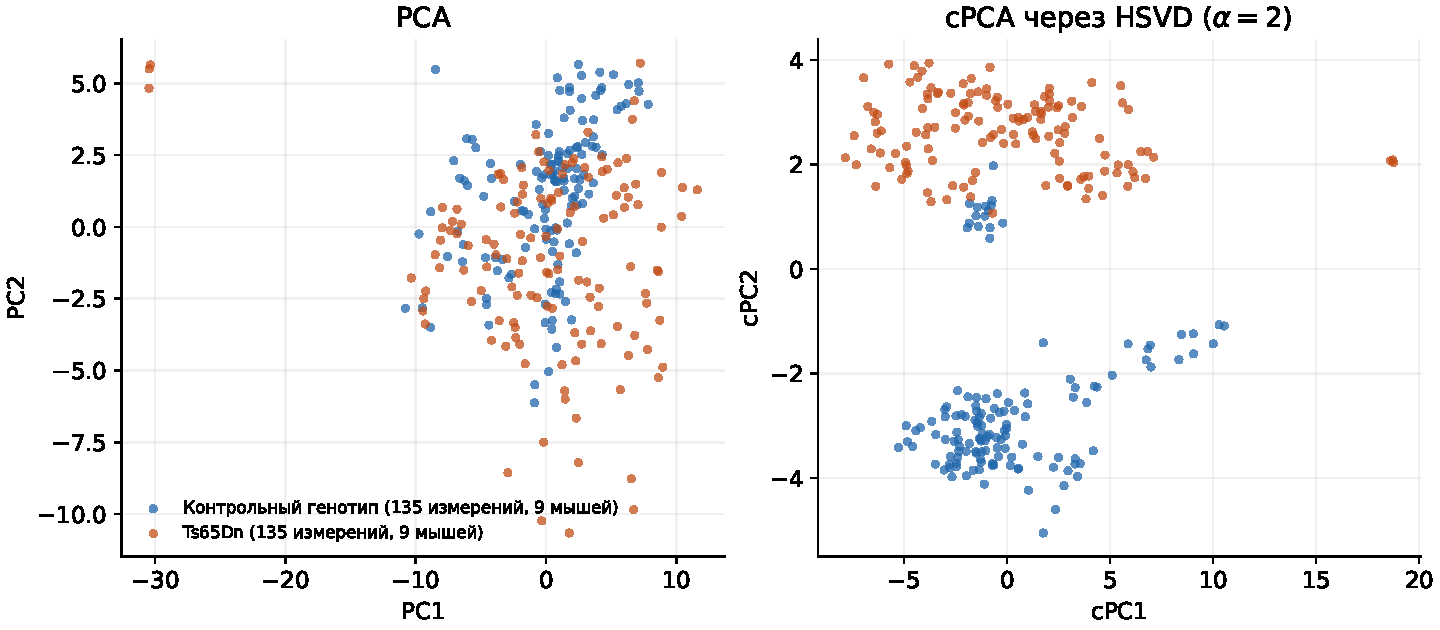
\includegraphics[width=1.00\linewidth]{pca_vs_cpca.pdf}
\caption{PCA и cPCA на реальных белковых данных. Синим обозначен контрольный
генотип, оранжевым --- Ts65Dn, по $135$ измерений у $9$ мышей.
Двумерная визуализация по образцу работы~\cite{cPCA}.}
\label{fig:app-cpca-realistic}
\end{figure}

В проекции cPCA группы разделяются заметнее, чем в PCA.
HSVD даёт то же подпространство, что и прямая диагонализация $H$,
с расхождением проекторов меньше $10^{-13}$.
\end{example}

\subsection{Наименьшие квадраты с неопределённой метрикой}
\textbf{Задача.}
Найти минимум $F(x)=(A^*x-b)^*J(A^*x-b)$,
где $b\in\HSVDComplex^n$, $x\in\HSVDComplex^m$, или установить, что его нет.

\textbf{Как используется HSVD.}
Вычисляем $z=U^*x$ и $\beta=V^{-1}b$. Тогда
\[
F(x)=(\Sigma^*z-\beta)^*J(\Sigma^*z-\beta).
\]
Каноническая $\Sigma$ разбивает задачу на независимые скалярные слагаемые:
положительные и отрицательные квадраты и нейтральные пары.
Каждая нейтральная пара превращается в линейный член:
\[
|z_i-\beta_i^+|^2-|z_i-\beta_i^-|^2
=2\operatorname{Re}\!\left(\overline{z_i}(\beta_i^--\beta_i^+)\right)
+\mathrm{const}.
\]
Отрицательный квадрат или ненулевой линейный член означает
неограниченность снизу. Иначе минимизируем положительные квадраты
по отдельности и возвращаемся к $x=Uz$.

\begin{proposition}[Условие существования минимума и все решения]
\label{prop:app-ils}
Положим $H=AJA^*$ и $g=AJb$. Минимум $F$ существует тогда и только тогда, когда
$H\succeq0$ и $g\in\im H$. При выполнении этих условий
\[
\mathop{\rm argmin}_x F(x)=H^\dagger g+\ker H,
\qquad
\min_x F(x)=b^*Jb-g^*H^\dagger g,
\]
где $H^\dagger$ --- псевдообратная матрица Мура--Пенроуза.
Точка минимума единственна тогда и только тогда, когда $H\succ0$.
Если хотя бы одно из условий существования нарушено, то
$\inf_x F(x)=-\infty$.
\end{proposition}
\begin{proof}
Раскроем скобки:
\[
F(x)=x^*Hx-2\operatorname{Re}(x^*g)+b^*Jb.
\]
Если $Hv=\lambda v$ и $\lambda<0$, то при $x=tv$, $t\in\mathbb R$,
отрицательный квадратичный член даёт $F(tv)\to-\infty$.
Пусть $H\succeq0$, но $g\notin\im H=(\ker H)^\perp$.
Ортогональная проекция $g_0$ вектора $g$ на $\ker H$ ненулевая,
и $F(tg_0)=b^*Jb-2t\|g_0\|_2^2\to-\infty$ при $t\to+\infty$.
Наконец, при выполнении обоих условий $x_0=H^\dagger g$ удовлетворяет
$Hx_0=g$, поэтому
\[
F(x)=(x-x_0)^*H(x-x_0)+b^*Jb-g^*H^\dagger g.
\]
Первое слагаемое неотрицательно и равно нулю ровно при
$x-x_0\in\ker H$. Это даёт все точки минимума и условие единственности.
\end{proof}

\textbf{Сравнение.}
HSVD явно показывает вырожденные направления и причину отсутствия минимума.
Тот же анализ можно провести по $H=AJA^*$ и $AJb$.
Если требуется только решение задачи с $H\succ0$,
гиперболический QR~\cite{ILS}
позволяет обойтись без полного спектрального разложения.


\subsection{Оптимальное сжатие матрицы Грама}
\textbf{Задача.}
Приблизить $H=AJA^*$ представлением $BJB^*$,
где $B\in\HSVDComplex^{m\times n}$, $\rank B\le k$,
$0\le k<\rank H$.

Задача возникает, например, для разности ковариационных матриц
двух состояний системы $H=XX^*-YY^*$.
Здесь $A=(X\;Y)$ и $J=\diag(I,-I)$.
Положительные и отрицательные собственные значения $H$ описывают
увеличение и уменьшение дисперсии вдоль соответствующих направлений.

\textbf{Как выбирается приближение $B_k$.}
Используем $H=U\Lambda U^*$, где $\Lambda=\Sigma J\Sigma^*$.
Упорядочим собственные значения $H$ по убыванию модуля
и обозначим соответствующие столбцы $U$ через $u_1,\ldots,u_m$.
Положим $U_k=(u_1,\ldots,u_k)$.
Эти направления описывают самые большие по модулю изменения,
включая как положительные, так и отрицательные значения.

Матрица $P_k=U_kU_k^*$ --- ортогональный проектор на выбранное
подпространство. Применим его к каждому столбцу исходной матрицы:
\[
B_k=P_kA=U_k(U_k^*A)=\sum_{i=1}^{k}u_i(u_i^*A).
\]
Таким образом, каждый столбец $A$ заменяется своей проекцией
на одни и те же $k$ направлений. Размер $B_k$ остаётся $m\times n$,
но её ранг не превосходит $k$.
Для хранения $B_k$ достаточно двух матриц: $U_k$ размера $m\times k$
и $R_k=U_k^*A$ размера $k\times n$.
Для самой матрицы Грама достаточно $U_k$ и $k$ собственных значений,
то есть $mk+k$ чисел:
\[
H_k=B_kJB_k^*=U_k\diag(\lambda_1,\ldots,\lambda_k)U_k^*.
\]
В канонической форме HSVD это соответствует сохранению
строк $\Sigma$ для выбранных ненулевых собственных значений
и обнулению остальных строк, включая нейтральные.

\begin{proposition}[Лучшее приближение матрицы Грама заданного ранга]
\label{prop:app-compression}
Для $|\lambda_1|\ge\cdots\ge|\lambda_m|$ построенная матрица $B_k$
достигает точного минимума
\[
\min_{\rank B\le k}\|AJA^*-BJB^*\|_F^2
=\sum_{i=k+1}^{m}\lambda_i^2.
\]
\end{proposition}
\begin{proof}
Любая $BJB^*$ имеет ранг не выше $k$, поэтому её погрешность не меньше
погрешности лучшего приближения $H$ ранга не выше $k$.
По теореме Эккарта--Янга--Мирского~\cite{Golub} квадрат этой погрешности
равен сумме квадратов отброшенных сингулярных чисел.
Для эрмитовой $H$ сингулярные числа равны $|\lambda_i|$.
С другой стороны, $\rank B_k\le k$, и
\[
B_kJB_k^*=U_kU_k^*HU_kU_k^*
=U_k\diag(\lambda_1,\ldots,\lambda_k)U_k^*.
\]
По унитарной инвариантности нормы Фробениуса квадрат погрешности равен
$\sum_{i=k+1}^{m}\lambda_i^2$.
При $k=0$ берём $B_0=0$. Следовательно, нижняя граница достигается.
\end{proof}

Для относительной ошибки не выше заданного $\delta>0$ выбирают
наименьшее $k$, для которого
\[
\sum_{i=k+1}^{m}\lambda_i^2\le\delta^2\sum_{i=1}^{m}\lambda_i^2.
\]
Если такого $k<\rank H$ нет, уменьшить ранг с этой точностью нельзя.
Усечение спектрального разложения $H$ даёт тот же результат, но HSVD позволяет построить это приближение непосредственно из матрицы $A$.


\section*{Заключение}
\phantomsection
\addcontentsline{toc}{section}{Заключение}

В работе исследовано гиперболическое сингулярное разложение произвольной
прямоугольной матрицы. Теорема существования HSVD, а также связь с собственными и присоединёнными векторами вспомогательных матриц были известны~\cite{Shirokov}, однако здесь предложены два варианта доказательства теоремы существования (неконструктивное через теорему Витта
и с помощью явного построения всех факторов разложения), которые лучше раскрывают структуру HSVD и позволяют строить алгоритмы для его вычисления.
На основе второго доказательства построен и реализован общий алгоритм,
который учитывает неполный ранг и нейтральные блоки, но не формирует явно матрицы Грама и не вычисляет жорданову форму.

Показано, что средняя матрица содержит
не менее $r+j$ ненулевых элементов и столбцов (в частности, это значит, что она не может быть диагональной в общем случае), а каноническая форма~(\ref{eq:canonical})
достигает этой границы. Исследована чувствительность параметра
$j=\rank(A)-\rank(AJA^*)$.
При полном ранге он сохраняется при достаточно малых возмущениях
только в случае $j=0$, при неполном ранге значение $j>0$ неустойчиво,
а при $j=0$ возможны оба варианта поведения.

Для гиперболических сингулярных чисел получены оценки погрешности
и формула для числа обусловленности в случае простого собственного значения.
Установлена связь обратной ошибки с невязками и нормой матрицы $V$.
Эти оценки показывают, почему малой невязки недостаточно для точного определения
ранга и малых гиперболических сингулярных чисел.

Численные эксперименты подтвердили работоспособность реализации
на проверенных матрицах разной структуры. На матрицах полного
столбцового ранга общий алгоритм оказался быстрее использованного
прототипа гиперболического метода Якоби. На тестах с большим разбросом гиперболических
сингулярных чисел преимущество по точности было у Якоби. Вблизи вырожденных направлений выбор численного
ранга остаётся чувствительным к порогам, поэтому общую устойчивость
алгоритма эти эксперименты не устанавливают.

Предложены способы применения HSVD в известных задачах cPCA, наименьших квадратов с неопределённой метрикой
и приближения матрицы Грама.
Для cPCA построены проекции открытых данных об измерениях белков.
Найденное подпространство cPCA совпало с результатом прямой диагонализации матрицы разности ковариаций.
Вклад работы в эти приложения состоит в их разборе через HSVD и воспроизводимой реализации примера cPCA.

\newpage

\phantomsection
\addcontentsline{toc}{section}{Список литературы}

\begin{thebibliography}{99}
\raggedright
\bibitem{Tyrtyshnikov}
Тыртышников, Е.~Е.
Матричный анализ и линейная алгебра [Электронный ресурс] /
Е.~Е.~Тыртышников. --- М., 2004--2005. ---
URL: \url{https://www.inm.ras.ru/wp-content/uploads/library/Monographies/all.pdf}
(дата обращения: 15.10.2026).

\bibitem{cPCACode}
Abid, A.
Contrastive PCA: авторская реализация и демонстрационные ноутбуки
[Электронный ресурс]. ---
URL: \url{https://github.com/abidlabs/contrastive}
(дата обращения: 15.10.2026).

\bibitem{cPCA}
Abid, A.
Exploring patterns enriched in a dataset with contrastive principal component
analysis / A.~Abid, M.~J.~Zhang, V.~K.~Bagaria, J.~Zou //
Nature Communications. --- 2018. --- Vol.~9. --- Art.~2134. ---
DOI: \href{https://doi.org/10.1038/s41467-018-04608-8}{10.1038/s41467-018-04608-8}.

\bibitem{ACM}
Association for Computing Machinery.
How to Classify Works Using ACM's Computing Classification System
[Электронный ресурс]. --- 2015. --- 5~с. ---
URL: \url{https://www.acm.org/binaries/content/assets/publications/article-templates/ccs-howto-v6-12jan2015.pdf}
(дата обращения: 13.10.2026).

\bibitem{BOS}
Bojanczyk, A.~W.
Existence of the hyperbolic singular value decomposition /
A.~W.~Bojanczyk, R.~Onn, A.~O.~Steinhardt //
Linear Algebra and its Applications. --- 1993. ---
Vol.~185. --- P.~21--30. ---
DOI: \href{https://doi.org/10.1016/0024-3795(93)90202-Y}{10.1016/0024-3795(93)90202-Y}.

\bibitem{ILS}
Bojanczyk, A.
Solving the indefinite least squares problem by hyperbolic QR factorization /
A.~Bojanczyk, N.~J.~Higham, H.~Patel //
SIAM Journal on Matrix Analysis and Applications. --- 2003. ---
Vol.~24, no.~4. --- P.~914--931. ---
DOI: \href{https://doi.org/10.1137/S0895479802401497}{10.1137/S0895479802401497}.

\bibitem{WittHermitian}
Bolshakov, Y.
Extension of isometries in finite-dimensional indefinite scalar product
spaces and polar decompositions /
Y.~Bolshakov, C.~V.~M.~van der Mee, A.~C.~M.~Ran,
B.~Reichstein, L.~Rodman //
SIAM Journal on Matrix Analysis and Applications. --- 1997. ---
Vol.~18, no.~3. --- P.~752--774. ---
DOI: \href{https://doi.org/10.1137/S0895479895290644}{10.1137/S0895479895290644}.

\bibitem{DavisKahan}
Davis, C.
The Rotation of Eigenvectors by a Perturbation.~III /
C.~Davis, W.~M.~Kahan //
SIAM Journal on Numerical Analysis. --- 1970. ---
Vol.~7, no.~1. --- P.~1--46. ---
DOI: \href{https://doi.org/10.1137/0707001}{10.1137/0707001}.

\bibitem{Drmac2021}
Drma\v{c}, Z.
Numerical methods for accurate computation of the eigenvalues of
Hermitian matrices and the singular values of general matrices /
Z.~Drma\v{c} //
SeMA Journal. --- 2021. --- Vol.~78, no.~1. --- P.~53--92. ---
DOI: \href{https://doi.org/10.1007/s40324-020-00229-8}{10.1007/s40324-020-00229-8}.

\bibitem{Golub}
Golub, G.~H.
Matrix Computations / G.~H.~Golub, C.~F.~Van Loan. ---
4th ed. --- Baltimore : Johns Hopkins University Press, 2013. ---
784~p. ---
DOI: \href{https://doi.org/10.56021/9781421407944}{10.56021/9781421407944}.

\bibitem{GreenbaumLiOverton2020}
Greenbaum, A.
First-Order Perturbation Theory for Eigenvalues and Eigenvectors /
A.~Greenbaum, R.-C.~Li, M.~L.~Overton //
SIAM Review. --- 2020. --- Vol.~62, no.~2. --- P.~463--482. ---
DOI: \href{https://doi.org/10.1137/19M124784X}{10.1137/19M124784X}.

\bibitem{FullBlockJJacobi}
Hari, V.
Full block J-Jacobi method for Hermitian matrices /
V.~Hari, S.~Singer, S.~Singer //
Linear Algebra and its Applications. --- 2014. ---
Vol.~444. --- P.~1--27. ---
DOI: \href{https://doi.org/10.1016/j.laa.2013.11.028}{10.1016/j.laa.2013.11.028}.

\bibitem{HariNovakovic2026}
Hari, V.
On Convergence and Accuracy of the J-Jacobi Method under the de Rijk
Pivot Strategy / V.~Hari, V.~Novakovi\'c //
Electronic Transactions on Numerical Analysis. --- 2026. ---
Vol.~65. --- P.~26--62. ---
DOI: \href{https://doi.org/10.1553/etna_vol65s26}{10.1553/etna\_vol65s26}.

\bibitem{HighamAccuracy}
Higham, N.~J.
Accuracy and Stability of Numerical Algorithms / N.~J.~Higham. ---
2nd ed. --- Philadelphia : SIAM, 2002. --- XXX, 680~p. ---
DOI: \href{https://doi.org/10.1137/1.9780898718027}{10.1137/1.9780898718027}.

\bibitem{MiceProtein}
Higuera, C.
Mice Protein Expression [Набор данных] / C.~Higuera, K.~Gardiner, K.~Cios. ---
UCI Machine Learning Repository, 2015. ---
DOI: \href{https://doi.org/10.24432/C50S3Z}{10.24432/C50S3Z}.

\bibitem{Higuera2015}
Higuera, C.
Self-Organizing Feature Maps Identify Proteins Critical to Learning in a
Mouse Model of Down Syndrome / C.~Higuera, K.~J.~Gardiner, K.~J.~Cios //
PLoS ONE. --- 2015. --- Vol.~10, no.~6. --- Article~e0129126. ---
DOI: \href{https://doi.org/10.1371/journal.pone.0129126}
{10.1371/journal.pone.0129126}.

\bibitem{Kalman}
Kalman, D.
A Singularly Valuable Decomposition: The SVD of a Matrix / D.~Kalman //
The College Mathematics Journal. --- 1996. --- Vol.~27, no.~1. ---
P.~2--23. ---
DOI: \href{https://doi.org/10.1080/07468342.1996.11973744}{10.1080/07468342.1996.11973744}.

\bibitem{Levy}
Levy, B.~C.
A note on the hyperbolic singular value decomposition / B.~C.~Levy //
Linear Algebra and its Applications. --- 1998. ---
Vol.~277, no.~1--3. --- P.~135--142. ---
DOI: \href{https://doi.org/10.1016/S0024-3795(98)10055-1}{10.1016/S0024-3795(98)10055-1}.

\bibitem{GPU-HSVD}
Novakovi\'c, V.
A GPU-based hyperbolic SVD algorithm / V.~Novakovi\'c, S.~Singer //
BIT Numerical Mathematics. --- 2011. --- Vol.~51, no.~4. ---
P.~1009--1030. ---
DOI: \href{https://doi.org/10.1007/s10543-011-0333-5}{10.1007/s10543-011-0333-5}.

\bibitem{AccJac}
Novakovi\'c, V.
AccJac: J-Jacobi method with accurate complex Jacobi rotations
[Электронный ресурс] / V.~Novakovi\'c. --- Исходный код программы. ---
URL: \url{https://github.com/venovako/AccJac}
(дата обращения: 15.10.2026).

\bibitem{Shirokov}
Shirokov, D.~S.
A note on the hyperbolic singular value decomposition without hyperexchange
matrices / D.~S.~Shirokov //
Journal of Computational and Applied Mathematics. --- 2021. ---
Vol.~391. --- Art.~113450. ---
DOI: \href{https://doi.org/10.1016/j.cam.2021.113450}{10.1016/j.cam.2021.113450}.

\bibitem{ShirokovYM}
Shirokov, D.~S.
Classification of all constant solutions of SU(2) Yang--Mills equations with
arbitrary current in pseudo-Euclidean space $\mathbb R^{p,q}$ /
D.~S.~Shirokov //
Modern Physics Letters A. --- 2023. --- Vol.~38, no.~20--21. ---
Art.~2350096. ---
DOI: \href{https://doi.org/10.1142/S0217732323500967}{10.1142/S0217732323500967}.

\bibitem{Jacobi}
Slapni\v{c}ar, I.
Highly accurate symmetric eigenvalue decomposition and hyperbolic SVD /
I.~Slapni\v{c}ar //
Linear Algebra and its Applications. --- 2003. ---
Vol.~358, no.~1--3. --- P.~387--424. ---
DOI: \href{https://doi.org/10.1016/S0024-3795(02)00516-5}{10.1016/S0024-3795(02)00516-5}.

\bibitem{TrefethenBauNLA}
Trefethen, L.~N.
Numerical Linear Algebra / L.~N.~Trefethen, D.~Bau~III. ---
Philadelphia : SIAM, 1997. --- XII, 361~p. ---
DOI: \href{https://doi.org/10.1137/1.9780898719574}{10.1137/1.9780898719574}.

\bibitem{Zha}
Zha, H.
A note on the existence of the hyperbolic singular value decomposition /
H.~Zha //
Linear Algebra and its Applications. --- 1996. ---
Vol.~240. --- P.~199--205. ---
DOI: \href{https://doi.org/10.1016/0024-3795(94)00197-9}{10.1016/0024-3795(94)00197-9}.

\end{thebibliography}

\end{document}
